\documentclass[11pt,a4paper]{article}

\usepackage[utf8x]{inputenc}   % omogoča uporabo slovenskih črk kodiranih v formatu UTF-8
\usepackage[slovene]{babel}    % naloži, med drugim, slovenske delilne vzorce

\usepackage[hyphens]{url}
\usepackage{hyperref}

\usepackage{graphicx}

\title{Prenos stila avtorja preko globokih nevronskih mrež\\
\textsc{dispozicija}}
\author{Aljoša Rakita\\
aljo.aljo.aljo@hotmail.com\\
\ \\
MENTOR: (prof.) dr. Franc Solina \\
Fakulteta za računalništvo in informatiko Univerze v Ljubljani
\date{\today}         
}


\begin{document}
\maketitle

\begin{abstract}
V tej diplomski nalogi, bo najprej razloženo kaj sploh globoke nevronske mreže so in kratka razlaga njihovega delovanja.


Nato bomo nekaj besed namenili temu, da bomo sploh ugotovili kako je stil slike definiran in kaj vse predstavlja.


Po tem, bomo natančno razložili in analizirali delovanje specifičnih metod za prenos stila slike preko globokih nevronskih mrež.


Zaključili bomo z demonstracijo delovanja in anketo, ki bo preverila kako realne so producirane slike.

\end{abstract}


\section{Motivacija za izbrano diplomsko temo}

Za to temo sem se odločil, ker se mi zdi področje umetne inteigence zelo zanimivo in perspektivno. Naloga bo razložila in analizirala sistem za prenos stila slike preko globokih nevronski mrež. Poleg tega bo služila tudi kot neka kritična ocena, kako sposobne so sodobne metode umetne inteligence ustvariti nekaj zelo človeškega: umetnost. 


Rezultati bodo koristili laikom, ža lažje razumevanje, kot tudi strokovnjakom za pomoč pri izbiri ustrezne metode.

\subsection{Pregled področja in sorodnih del}

\begin{itemize}
  \item Image style transfer using convolutional neural networks\cite{gatys2016image} : Predstavi sistem, ki temelji na globokih nevronskih mrežah, ki ustvari visoko-kvalitetne umetniške slike. Članek naredi korak naprej v razumevanju kako ljudje ustvarjamo in zaznavamo umetnost.
  \item Preserving color in neural artistic style transfer\cite{gatys2016preserving} : Nadaljevanje zgornjega članka, ki se loti problemov in pomankljivosti opisanega algoritma. Opiše preproste linearne metode, ki problem rešijo.
  \item Texture Networks: Feed-forward Synthesis of Textures and Stylized Images.\cite{ulyanov2016texture} : V tem članku je predstavljen sistem, ki hitreje ustvari sliko, saj je večina obdelave prestavljena v fazo učenja nevronskih mrež.


\end{itemize}


\subsection{Zakaj je predlagani mentor primeren}

Profesor doktor Franc Solina je predstojnk laboratorija za računlniški vid,
ki se ukvarja z raziskavami na istem področju, kot je tema te diplomske
naloge. Poleg tega je bil profesor mentor že velikemu številu študentov.



\section{Miselni diagram za izbrano temo diplomske naloge}

\begin{figure}[p]
\centerline{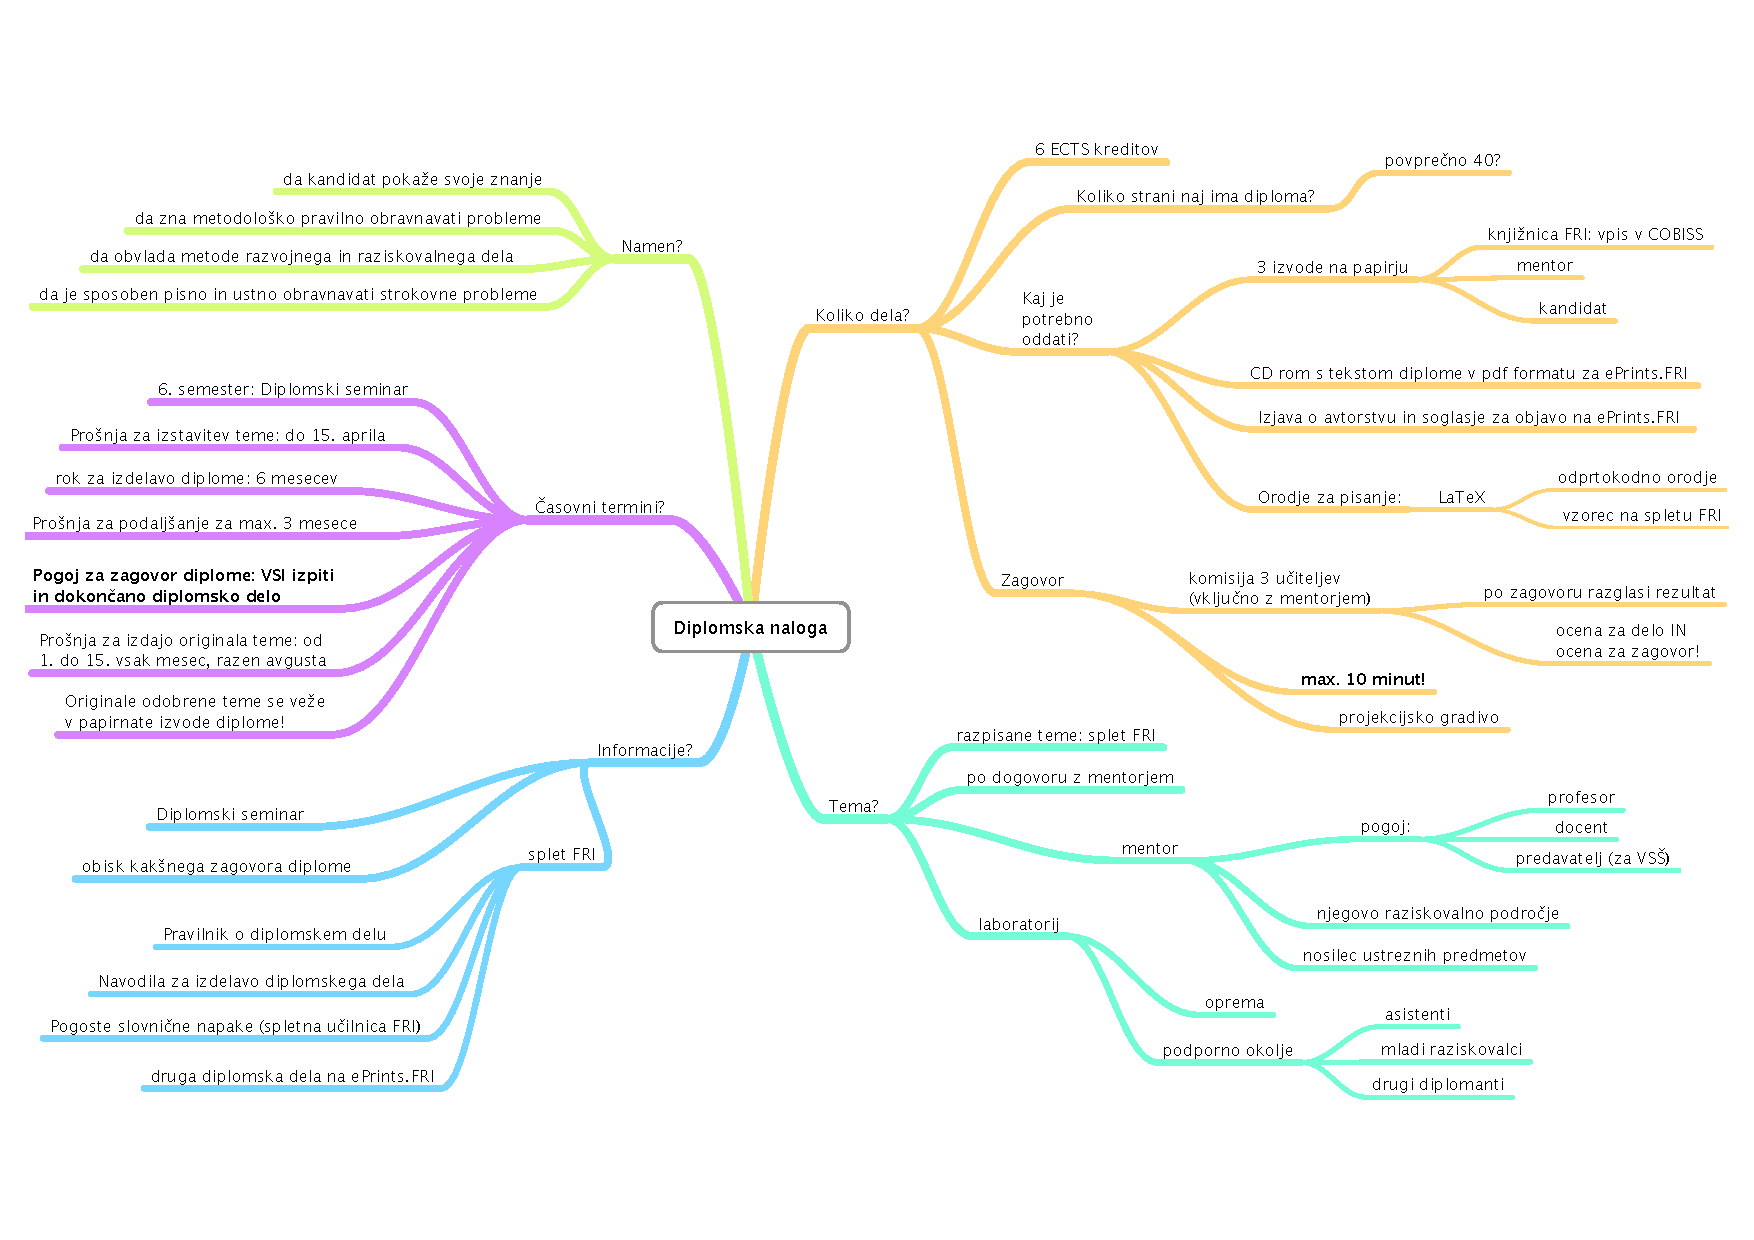
\includegraphics[height=1.0\textwidth, angle=90]{mindmap.pdf}}
\caption{Miselni vzorec za mojo diplomsko nalogo.}
\label{sl:mindmap}
\end{figure}

Na posebni strani je vključen dopolnjen miselni vzorec (Slika \ref{sl:mindmap}).



\section{Predvideni prispevki diplomske naloge}

Rezultat diplomske naloge bo analiza, razlaga ter primerjava metod za prenos stila slike. To bo vključevalo demonstracijo tega postopka na slikah pokrajine s pomočjo stila nekaterih slovenskih impresionistov in spletno anketo širše množice, ki bo ocenila ali so ljudje sposobni ločiti umetno od človeškega.


\section{Uporabljena metodologija}

V procesu izdelave diplomske naloge bom uporabil razvojno okolje PyCharm, saj so dostopne otprtokodne rešitve realizirane v programskem jeziku python in pa spletno platformo za izdelavo in objavo anket 1ka.

\section{Razdelitev potrebnega dela na aktivnosti}

\begin{enumerate}
  \item ideja za diplomo (konkreten razmislek o temi diplome; tema diplomskega dela) 1 mesec
  \item iskanje mentorja (sestanek v živo, pisanje emailov; mentor diplomskega dela) 1 teden
  \item \v{s}tudij literature (iskanje, branje, pisanje povzetkov; teoretična podlaga) 1 mesec
  \item pisanje dispozicije (pisanje; dispozicija) 1 teden
  \item kodiranje (kodiranje, testiranje; delujoč program) 2 tedna
  \item anketiranje (sestavljanje ankete, čakanje in analiza rezultatov; odziv javnosti) 2 tedna
  \item pisanje diplome (razmišlanje, pisanje, preverjanje; napisana diploma) 1 mesec
  \item zagovor(priprava na zagovor,zagovarjanje; opravljena diploma) 1 mesec
\end{enumerate}


Zgornje aktivnosti se seštejejo v 4 mesece in pol, poleg tega pa lahko večino opravljam vzporedno, kar postopek še skrajša. Zato menim, da mi čas ne bo delal problemov.


\section{Preliminarno kazalo}

\begin{enumerate}
  \item Uvod
  \item Globoke nevronske mreže - kaj sploh globoke nevronske mreže so in kratka razlaga njihovega delovanja.
  \item Stil - kako je stil slike definiran in kaj vse predstavlja.
  \item Prenos stila s pomočjo globokih nevronskim mrež - razlaga delovanja in primerjava metod.
  \item Implementacija sistema za prenos stila - implementacija obstoječe otprtokodne rešitve in kreiranje primerov slik.
  \item Anketiranje - izdelava in objava ankete
  \item Analiza in interpretacija rezultatov
  \item Zaključek
  \item Literatura
\end{enumerate}

\pagebreak

\section{Seznam literature}



\bibliographystyle{plain}
\bibliography{literatura}

\end{document}  




